\documentclass[../Main.tex]{subfiles}
\begin{document}
\section{Testing}
This section will analyze the performance of the four kind of JRPC request that are essential for the login and registration use cases of the system. The requests are crucial for facilitating communication between the SDK and executors, and their performance significantly affects the overall efficiency and user experience of the system.\\
\indent The four JRPC requests being analyzed are:
\begin{itemize}
  \item \textbf{AssignKeyCommitmentRequest}-The AssignKeyCommitmentRequest is a critical step that acts as an aggregator for executor signatures, paving the way for the subsequent AssignKeyRequest
  \item \textbf{AssignKeyRequest}-In the AssignKeyRequest, a user initiates the process of being registered within the system. The user provides their idToken and the signatures obtained from the AssignKeyCommitmentRequest to achieve consensus across the nodes
  \item \textbf{CommitmentRequest}-The CommitmentRequest is a request sent by a registered user who already exists within the system. Through this request, the user seeks to obtain aggregated signatures from the nodes, facilitating the subsequent ShareRequest process
  \item \textbf{ShareRequest}-The ShareRequest process is initiated by users who wish to retrieve their encrypted share of the cryptographic key. This encrypted share is a crucial component that allows users to reconstruct their encKey, which is necessary for secure authentication.
\end{itemize}
To assess the performance of JRPC requests, we will conduct thorough testing and gather data on response times, request rates, and throughput. The objective is to assess the system's performance under different loads and detect any bottlenecks or areas that require enhancement. Furthermore, we will assess the influence of various factors, including network latency and system resources, on the performance of JRPC requests.\\
\indent The performance analysis will offer valuable insights into the system's scalability and its capacity to handle a high volume of users and concurrent requests. Optimizing the performance of critical JRPC requests can enhance system responsiveness, reduce latency, and improve the user experience during login and registration.\\
To conduct tests, I utilize the autocannon\cite{autocannon} package, which can be executed directly in Node.js with the following hyperparameters:
\begin{itemize}
  \item Hyperparameters for autocannon:
    \begin{itemize}
      \item connections: 10, 100, 1000, 2000, 4000, 8000
      \item durations: 10s
      \item number of worker: 1
    \end{itemize}
  \item Hardware specification:
    \begin{itemize}
      \item Processor: Apple M1 Pro, 6 performance cores(600 - 3220 MHz) and 2 power efficiency core(600 - 2064 MHz)
      \item Memory: 16GB
    \end{itemize}
\end{itemize}

\subsection{CommitmentRequest}
\begin{table}[H]
\centering
\begin{tabular}{|l|l|l|l|l|l|l|l|}
\hline
\rowcolor[HTML]{f56b00}
\textbf{Stat} & \textbf{2.5\%} & \textbf{50\%} & \textbf{97.5\%} & \textbf{99\%} & \textbf{Avg} & \textbf{Stdev} & \textbf{Max} \\
\hline
Latency   & 0 ms  & 0 ms & 5 ms   & 8 ms & 0.93 ms & 2.08 ms & 71 ms \\
\hline
\rowcolor[HTML]{f56b00}
\textbf{Stat} & \textbf{1\%} & \textbf{2.5\%} & \textbf{50\%} & \textbf{97.5\%} & \textbf{Avg} & \textbf{Stdev} & \textbf{Min} \\
Req/Sec   & 4073  & 4073  & 6631   & 8359   & 6850.5  & 1134.82 & 4073  \\
\hline
Bytes/Sec & 5.66 MB & 5.66 MB & 9.22 MB & 11.6 MB & 9.52 MB & 1.58 MB & 5.66 MB \\
\hline
\end{tabular}
 \caption{10 connections performance}
 \label{10-connections-performance}
\end{table}

\begin{table}[H]
  \centering
\begin{tabular}{|l|l|l|l|l|l|l|l|}
\hline
\rowcolor[HTML]{f56b00}
\textbf{Stat} & \textbf{2.5\%} & \textbf{50\%} & \textbf{97.5\%} & \textbf{99\%} & \textbf{Avg} & \textbf{Stdev} & \textbf{Max} \\
\hline
Latency   & 4 ms  & 9 ms & 29 ms   & 36 ms & 10.66 ms & 8.48 ms & 406 ms \\
\hline
\rowcolor[HTML]{f56b00}
\textbf{Stat} & \textbf{1\%} & \textbf{2.5\%} & \textbf{50\%} & \textbf{97.5\%} & \textbf{Avg} & \textbf{Stdev} & \textbf{Min} \\
Req/Sec   & 5391   & 5391   & 9247    & 10647   & 8964.4  & 1496.42 & 5391    \\
\hline
Bytes/Sec & 7.5 MB & 7.5 MB & 12.9 MB & 14.8 MB & 12.5 MB & 2.08 MB & 7.49 MB \\
\hline
\end{tabular}
 \caption{100 connections performance}
 \label{100-connections-performance}
\end{table}

\begin{table}[H]
\centering
\begin{tabular}{|l|l|l|l|l|l|l|l|}
\hline
\rowcolor[HTML]{f56b00}
\textbf{Stat} & \textbf{2.5\%} & \textbf{50\%} & \textbf{97.5\%} & \textbf{99\%} & \textbf{Avg} & \textbf{Stdev} & \textbf{Max} \\
\hline
Latency & 26 ms & 57 ms & 134 ms & 284 ms & 97.63 ms & 461.09 ms & 9882 ms \\
\hline
\rowcolor[HTML]{f56b00}
\textbf{Stat} & \textbf{1\%} & \textbf{2.5\%} & \textbf{50\%} & \textbf{97.5\%} & \textbf{Avg} & \textbf{Stdev} & \textbf{Min} \\
Req/Sec & 3837 & 3837 & 9607 & 10495 & 8381.9 & 2219.44 & 3836 \\
\hline
Bytes/Sec & 5.33 MB & 5.33 MB & 13.4 MB & 14.6 MB & 11.6 MB & 3.09 MB & 5.33 MB \\
\hline
\end{tabular}
 \caption{1000 connections performance}
 \label{1000-connections-performance}
\end{table}

\begin{table}[H]
\centering
\begin{tabular}{|l|l|l|l|l|l|l|l|}
\hline
\rowcolor[HTML]{f56b00}
\textbf{Stat} & \textbf{2.5\%} & \textbf{50\%} & \textbf{97.5\%} & \textbf{99\%} & \textbf{Avg} & \textbf{Stdev} & \textbf{Max} \\
\hline
Latency (ms) & 177 & 273 & 1961 & 2454 & 436.85 & 434.88 & 2551 \\
\hline
\rowcolor[HTML]{f56b00}
\textbf{Stat} & \textbf{1\%} & \textbf{2.5\%} & \textbf{50\%} & \textbf{97.5\%} & \textbf{Avg} & \textbf{Stdev} & \textbf{Min} \\
\hline
Req/Sec & 361 & 361 & 1582 & 4531 & 2246.6 & 1550.91 & 361 \\
\hline
Bytes/Sec & 330 kB & 330 kB & 1.44 MB & 4.14 MB & 2.05 MB & 1.42 MB & 330 kB \\
\hline
\end{tabular}
 \caption{2000 connections performance}
 \label{2000-connections-performance}
\end{table}


\begin{table}[H]
   \centering
\begin{tabular}{|l|l|l|l|l|l|l|l|}
\hline
\rowcolor[HTML]{f56b00}
\textbf{Stat} & \textbf{2.5\%} & \textbf{50\%} & \textbf{97.5\%} & \textbf{99\%} & \textbf{Avg} & \textbf{Stdev} & \textbf{Max} \\
\hline
Latency (ms) & 194 & 417 & 2923 & 3688 & 611.3 & 578.23 & 4015 \\
\hline
\rowcolor[HTML]{f56b00}
\textbf{Stat} & \textbf{1\%} & \textbf{2.5\%} & \textbf{50\%} & \textbf{97.5\%} & \textbf{Avg} & \textbf{Stdev} & \textbf{Min} \\
\hline
Req/Sec & 1975 & 1975 & 3379 & 3779 & 3026.6 & 683.61 & 1975 \\
\hline
Bytes/Sec & 1.8 MB & 1.8 MB & 3.08 MB & 3.45 MB & 2.76 MB & 624 kB & 1.8 MB \\
\hline
\end{tabular}
 \caption{4000 connections performance}
 \label{4000-connections-performance} \end{table}


\begin{table}[H]
  \centering
\begin{tabular}{|l|l|l|l|l|l|l|l|}
\hline
\rowcolor[HTML]{f56b00}
\textbf{Stat} & \textbf{2.5\%} & \textbf{50\%} & \textbf{97.5\%} & \textbf{99\%} & \textbf{Avg} & \textbf{Stdev} & \textbf{Max} \\
\hline
Latency (ms) & 167 & 1672 & 5490 & 5668 & 2095.88 & 1205.08 & 5740 \\
\hline
\rowcolor[HTML]{f56b00}
\textbf{Stat} & \textbf{1\%} & \textbf{2.5\%} & \textbf{50\%} & \textbf{97.5\%} & \textbf{Avg} & \textbf{Stdev} & \textbf{Min} \\
\hline
Req/Sec & 185 & 185 & 364 & 802 & 472.9 & 216.68 & 185 \\
\hline
Bytes/Sec & 169 kB & 169 kB & 333 kB & 733 kB & 432 kB & 198 kB & 169 kB \\
\hline
\end{tabular}
 \caption{8000 connections performance}
 \label{8000-connections-performance}
\end{table}

\begin{figure}[H]
  \centering
  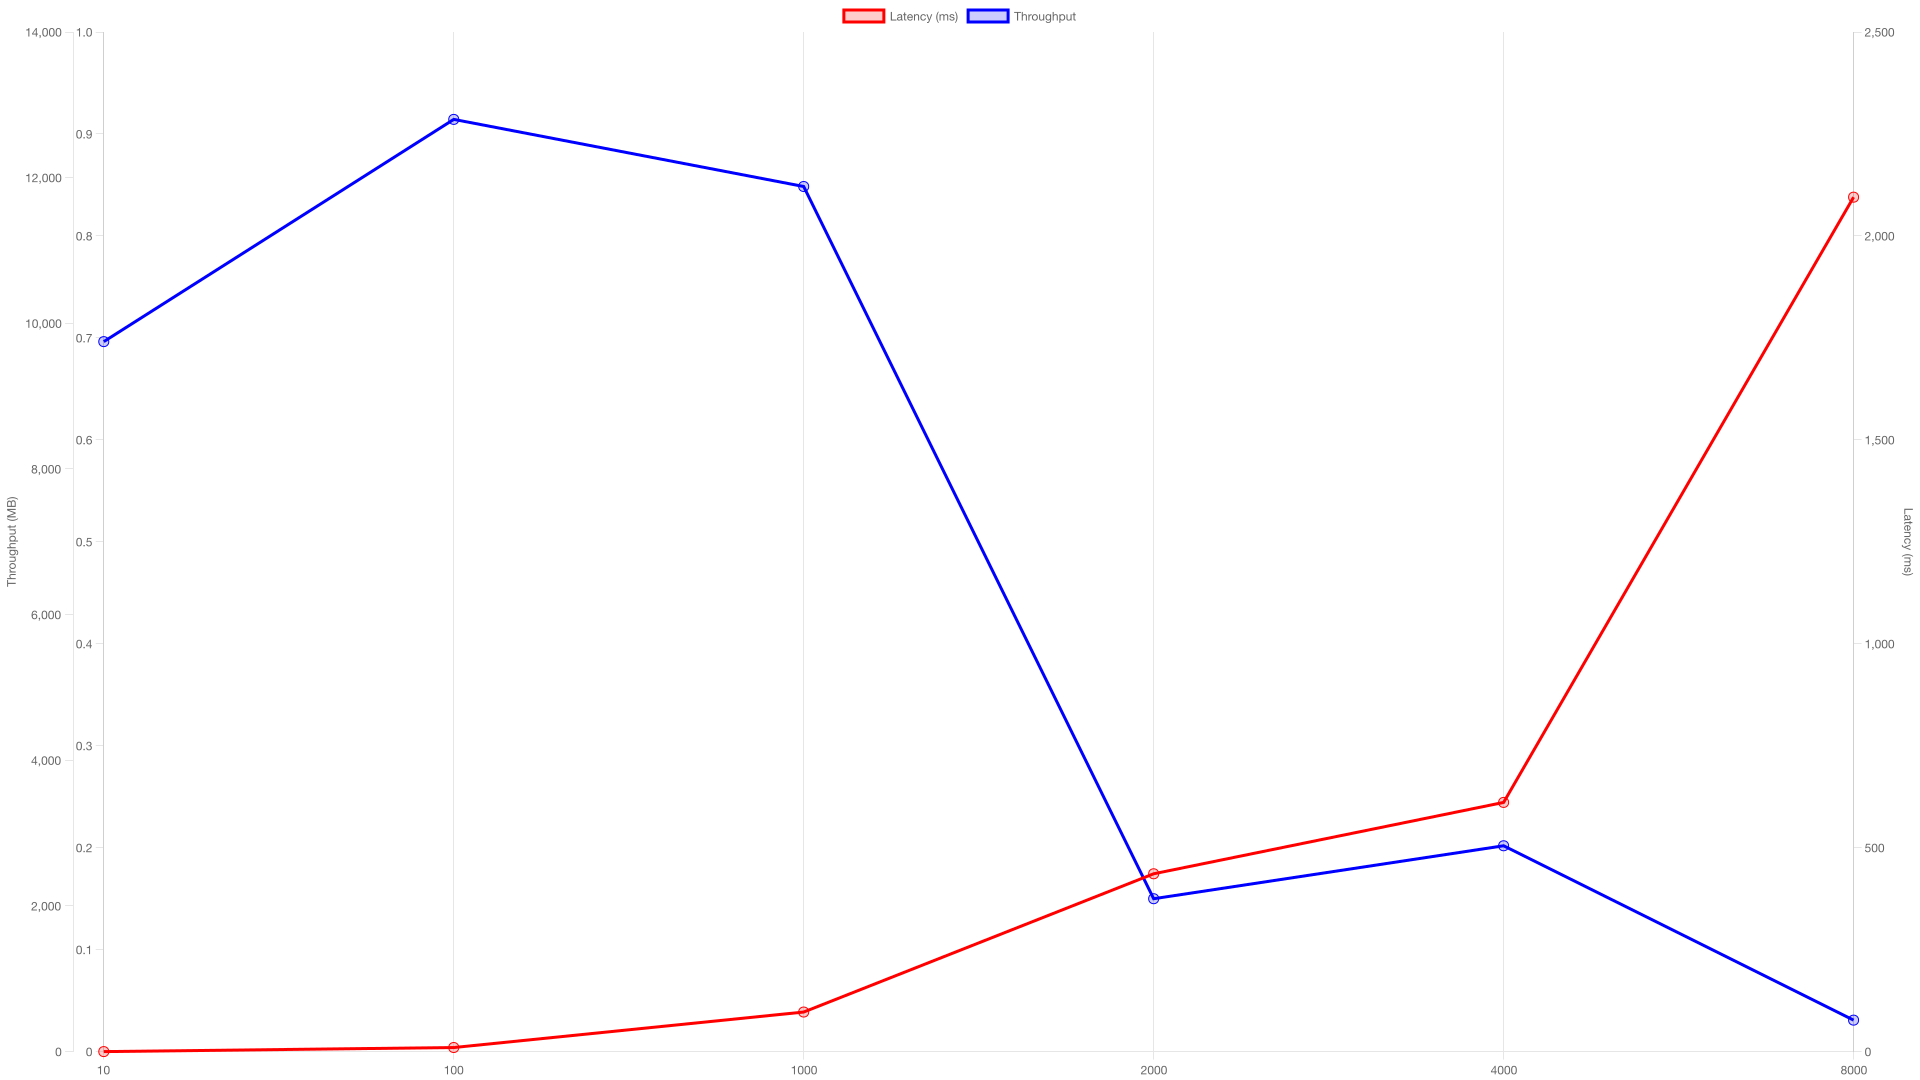
\includegraphics[scale=0.22]{Figure/commitments-line-chart.png}
  \caption{Commitment request latency and throughput line chart}
  \label{fig:commitments-line-chart}
\end{figure}
The provided data provides insightful insights into the performance analysis of various connection types. The analysis includes key metrics such as latency, request per second (req/sec), and throughput, which cast light on the server's efficiency and responsiveness under different conditions. The latency, or the time it takes for a request to travel from the client to the server and return, is a crucial indicator of the responsiveness of a system. The 2.5th percentile and median latency values represent the latency encountered by the quickest 2.5\% and median requests, respectively. The 97.5th and 99th percentiles, on the other hand, represent the latency for the majority of requests, with only a minor fraction experiencing higher latencies. The average latency provides a comprehensive view of the system's response time, whereas the standard deviation indicates the variation in latency values. The maximum latency represents the response time at its apex, as measured during the analysis. The request per second (req/sec) metric gauges the server's ability to process incoming requests. The values for the 1st and 2.5th percentiles represent the slowest 1\% and 2.5\% of observed requests, respectively. \\
\indent The median value indicates the rate at which half of the requests were processed, while the 97.5th percentile represents the rate at which the majority of requests were processed. The average req/sec across all connections provides an aggregate measure of the server's performance, whereas the standard deviation illustrates the processing capacity variation of the server. Throughput, which is measured in megabytes per second (MB/s), represents the quantity of data transmitted or received per second. Similar to the latency and req/sec values, the 2.5th percentile, median, 97.5th percentile, 99th percentile, average, standard deviation, and maximum values represent various aspects of the data transmission efficacy. This data analysis helps determine the performance characteristics of the system under various connection conditions. Lower latency values indicate quicker response times and a superior user experience, with the 2.5th percentile and median latencies being especially significant for the majority of user interactions. Higher latency percentiles may indicate intermittent performance issues or congestion during peak usage periods. In the meantime, higher req/sec values indicate a server's ability to process more requests concurrently, allowing for more fluid user interactions during periods of high traffic. The standard deviation values for latency and req/sec demonstrate the performance variance. The smaller the standard deviation, the more consistent and predictable the performance. Monitoring throughput is essential for determining the efficacy of data transmission, with higher throughput values indicating superior data exchange.

\begin{table}[H]
\subsection{ShareRequest}
  \centering
\begin{tabular}{|l|l|l|l|l|l|l|l|}
\hline
\rowcolor[HTML]{f56b00}
\textbf{Stat} & \textbf{2.5\%} & \textbf{50\%} & \textbf{97.5\%} & \textbf{99\%} & \textbf{Avg} & \textbf{Stdev} & \textbf{Max} \\
\hline
Latency   & 325 ms & 465 ms & 1130 ms & 1289 ms & 497.26 ms & 177.23 ms & 1307 ms \\
\hline
\rowcolor[HTML]{f56b00}
\textbf{Stat} & \textbf{1\%} & \textbf{2.5\%} & \textbf{50\%} & \textbf{97.5\%} & \textbf{Avg} & \textbf{Stdev} & \textbf{Min} \\
Req/Sec   & 10  & 10  & 19   & 28   & 19.5  & 5.38 & 10  \\
\hline
Bytes/Sec & 13 kB & 13 kB & 24.8 kB & 36.5 kB & 25.4 kB & 7.01 kB & 13 kB \\
\hline
\end{tabular}
 \caption{10 connections performance}
 \label{10-connections-performance}
\end{table}

\begin{table}[H]
  \centering
\begin{tabular}{|l|l|l|l|l|l|l|l|}
\hline
\rowcolor[HTML]{f56b00}
\textbf{Stat} & \textbf{2.5\%} & \textbf{50\%} & \textbf{97.5\%} & \textbf{99\%} & \textbf{Avg} & \textbf{Stdev} & \textbf{Max} \\
\hline
Latency   & 1751 ms & 3888 ms & 5850 ms & 5937 ms & 3843.44 ms & 990.28 ms & 6059 ms \\
\hline
\rowcolor[HTML]{f56b00}
\textbf{Stat} & \textbf{1\%} & \textbf{2.5\%} & \textbf{50\%} & \textbf{97.5\%} & \textbf{Avg} & \textbf{Stdev} & \textbf{Min} \\
Req/Sec   & 0  & 0  & 19   & 32   & 20.6  & 9.67 & 12  \\
\hline
Bytes/Sec & 0 B & 0 B & 24.8 kB & 41.8 kB & 26.9 kB & 12.6 kB & 15.6 kB \\
\hline
\end{tabular}
 \caption{100 connections performance}
 \label{100-connections-performance}
\end{table}

\begin{table}[H]
  \centering
\begin{tabular}{|l|l|l|l|l|l|l|l|}
\hline
\rowcolor[HTML]{f56b00}
\textbf{Stat} & \textbf{2.5\%} & \textbf{50\%} & \textbf{97.5\%} & \textbf{99\%} & \textbf{Avg} & \textbf{Stdev} & \textbf{Max} \\
\hline
Latency   & 1458 ms & 5752 ms & 9791 ms & 9924 ms & 5604.38 ms & 2517.41 ms & 9982 ms \\
\hline
\rowcolor[HTML]{f56b00}
\textbf{Stat} & \textbf{1\%} & \textbf{2.5\%} & \textbf{50\%} & \textbf{97.5\%} & \textbf{Avg} & \textbf{Stdev} & \textbf{Min} \\
Req/Sec   & 0  & 0  & 25   & 35   & 24.3  & 8.88 & 22  \\
\hline
Bytes/Sec & 0 B & 0 B & 32.6 kB & 45.7 kB & 31.7 kB & 11.6 kB & 28.7 kB \\
\hline
\end{tabular}
 \caption{1000 connections performance}
 \label{1000-connections-performance}
\end{table}

\begin{table}[H]
\centering
\begin{tabular}{|l|l|l|l|l|l|l|l|}
\hline
\rowcolor[HTML]{f56b00}
\textbf{Stat} & \textbf{2.5\%} & \textbf{50\%} & \textbf{97.5\%} & \textbf{99\%} & \textbf{Avg} & \textbf{Stdev} & \textbf{Max} \\ \hline
Latency & 2160 ms & 3892 ms & 9133 ms & 9575 ms & 4345.31 ms & 1799.95 ms & 10035 ms \\ \hline
\rowcolor[HTML]{f56b00}
\textbf{Stat} & \textbf{1\%} & \textbf{2.5\%} & \textbf{50\%} & \textbf{97.5\%} & \textbf{Avg} & \textbf{Stdev} & \textbf{Min} \\ \hline
Req/Sec & 3 & 3 & 178 & 247 & 158.81 & 79.46 & 3 \\ \hline
Bytes/Sec & 2.81 kB & 2.81 kB & 162 kB & 225 kB & 145 kB & 72.3 kB & 2.81 kB \\ \hline
\end{tabular}
 \caption{2000 connections performance}
 \label{2000-connections-performance}
\end{table}

\begin{table}[H]
  \centering
\begin{tabular}{|l|l|l|l|l|l|l|l|}
\hline
\rowcolor[HTML]{f56b00}
\textbf{Stat} & \textbf{2.5\%} & \textbf{50\%} & \textbf{97.5\%} & \textbf{99\%} & \textbf{Avg} & \textbf{Stdev} & \textbf{Max} \\ \hline
Latency (ms) & 2234 ms & 5475 ms & 9720 ms & 9995 ms & 5488.23 ms & 2227.17 ms & 10145 ms \\ \hline
\rowcolor[HTML]{f56b00}
\textbf{Stat} & \textbf{1\%} & \textbf{2.5\%} & \textbf{50\%} & \textbf{97.5\%} & \textbf{Avg} & \textbf{Stdev} & \textbf{Min} \\ \hline
Req/Sec & 2 & 2 & 83 & 177 & 84.6 & 50.73 & 2 \\ \hline
Bytes/Sec & 1.82 kB & 1.82 kB & 75.6 kB & 161 kB & 77 kB & 46.2 kB & 1.82 kB \\ \hline
\end{tabular}
 \caption{4000 connections performance}
 \label{4000-connections-performance}
\end{table}


\begin{table}[H]
\centering
\caption{Latency, Request Rate, and Throughput (Continued)}
\begin{tabular}{|l|l|l|l|l|l|l|l|}
\hline
\rowcolor[HTML]{f56b00}
\textbf{Stat} & \textbf{2.5\%} & \textbf{50\%} & \textbf{97.5\%} & \textbf{99\%} & \textbf{Avg} & \textbf{Stdev} & \textbf{Max} \\ \hline
Latency (ms) & 4632 ms & 7469 ms & 9732 ms & 9867 ms & 7255.9 ms & 1362.87 ms & 10151 ms \\ \hline
\rowcolor[HTML]{f56b00}
\textbf{Stat} & \textbf{1\%} & \textbf{2.5\%} & \textbf{50\%} & \textbf{97.5\%} & \textbf{Avg} & \textbf{Stdev} & \textbf{Min} \\ \hline
Req/Sec & 0 & 0 & 62 & 234 & 66.7 & 71.33 & 2 \\ \hline
Bytes/Sec & 0 B & 0 B & 56.4 kB & 215 kB & 60.9 kB & 65.5 kB & 1.82 kB \\ \hline
\end{tabular}
 \caption{8000 connections performance}
 \label{8000-connections-performance}
\end{table}

\begin{figure}[H]
  \centering
  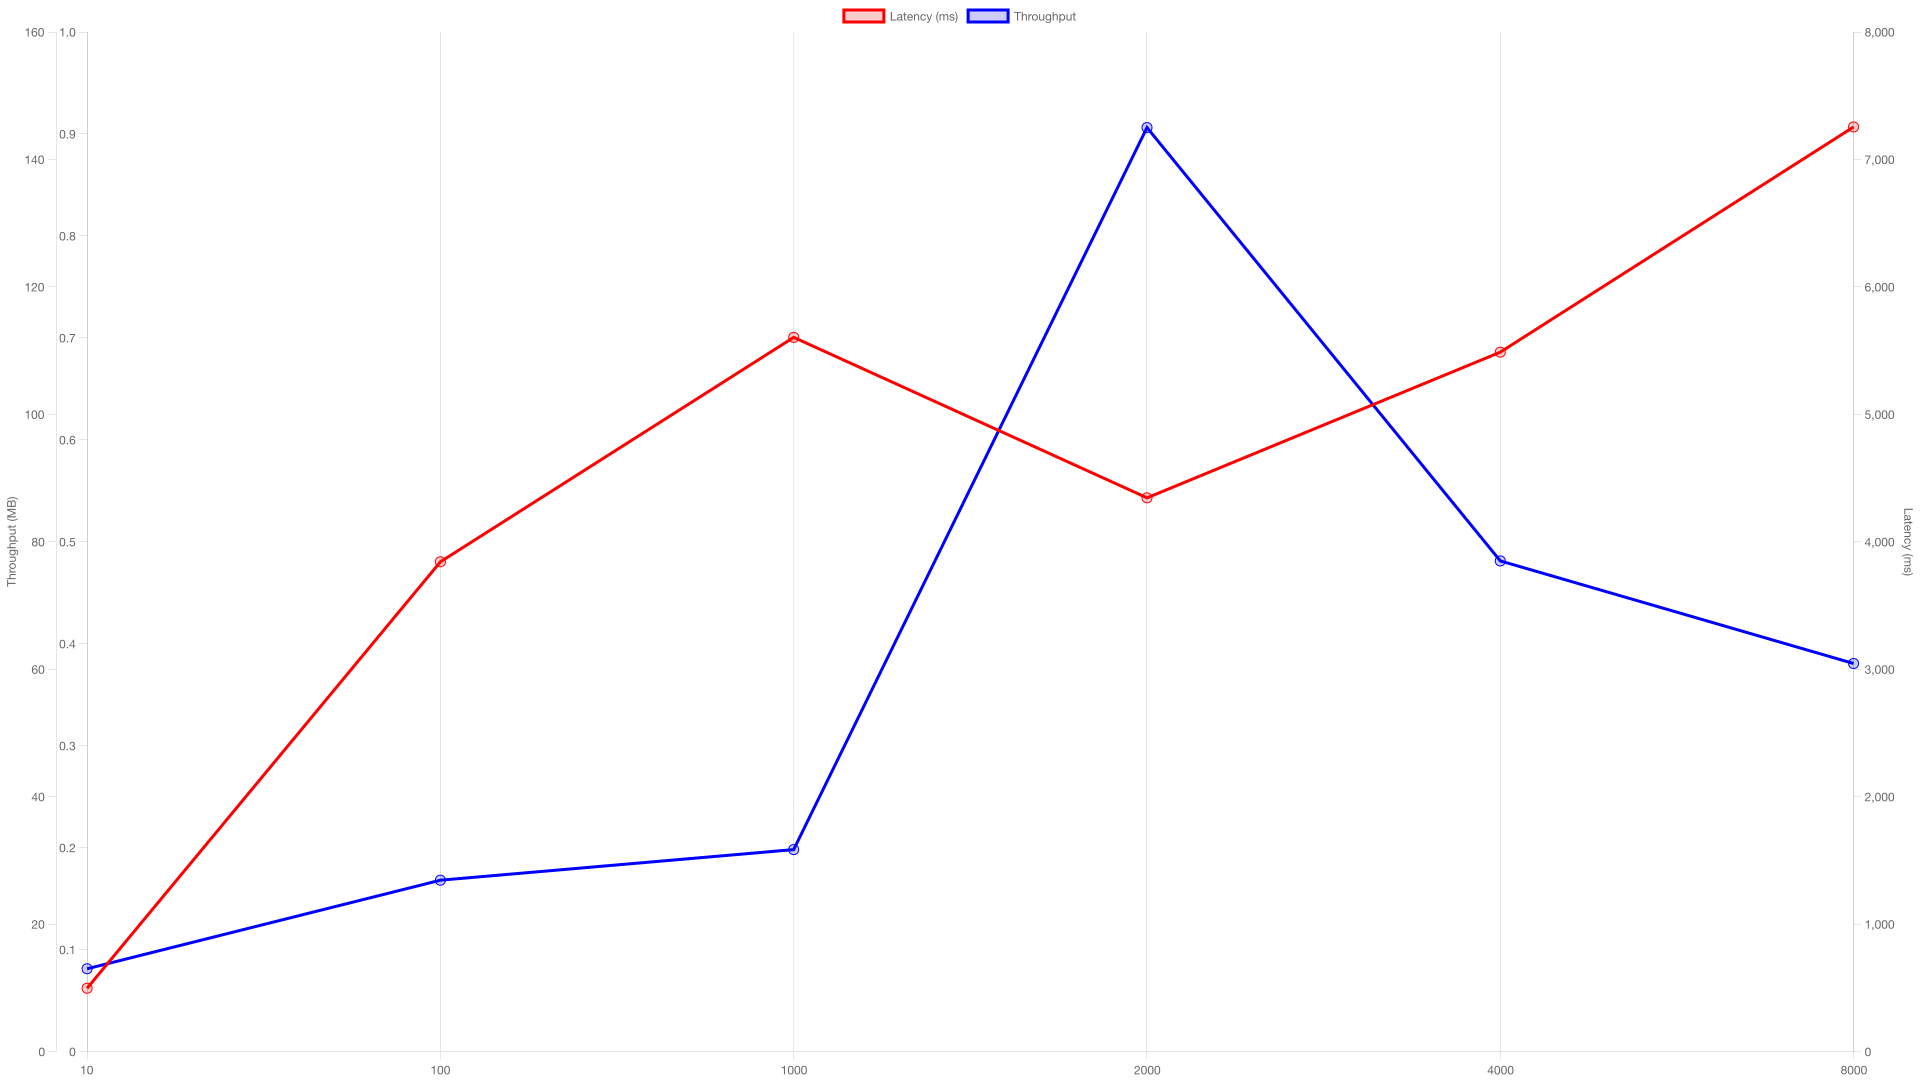
\includegraphics[scale=0.22]{Figure/sharerequest-line-chart.png}
  \caption{Share request latency and throughput line chart}
  \label{fig:sharerequest-line-chart}
\end{figure}

The dataset contains performance metrics for numerous connection types, ranging from ten to eight thousand connections. These metrics provide invaluable insights into the system's performance, and they are essential for comprehending its responsiveness and capacity under varying burdens. The 2.5th percentile latency ranges from approximately 325 ms to 4632 ms, indicating that only a small percentage of queries experience extremely quick response times. The median latency at the 50th percentile ranges from 465 milliseconds to 7469 milliseconds, representing typical response times for the majority of queries. The 97.5th percentile latency, between 1130 and 9732 milliseconds, represents the response time experienced by the vast majority of requests, comprising a wider range of response times. Similarly, the 99th percentile latency ranges from 1289 ms to 9867 ms, capturing the response time for an even higher percentage of requests, including some outliers. The range of 497.26 ms to 7255.9 ms for the average latency represents the response time of the system. The standard deviation of latency ranges from 177.23 ms to 1362.87 ms, indicating the variance in response times across queries. In conclusion, the maximal latency ranges from 1307 ms to 10151 ms, representing the longest response time observed throughout the analysis. Next, the 1st and 2.5th percentile values for req/sec are typically low or even negative, indicating that only a small fraction of requests experience the slowest processing rates or may be affected by problems resulting in no response. The median req/sec values range between 19 and 62, representing the rate at which half of the queries were processed. The 97.5th percentile req/sec ranges from 28 to 234 and represents the rate at which the preponderance of requests are processed. The average req/sec ranges from 19.5 to 66.7, providing an aggregate measure of the system's ability to handle incoming requests. The range of the standard deviation of req/sec from 5.38 to 71.33 exemplifies the variability of processing rates.\\
\indent The 2.5th percentile throughput values are generally low, ranging between 13 kilobytes and zero bytes, indicating slower data transmission rates for certain queries. The median throughput, which is equal to the 50th percentile, ranges from 13 kB to 0 B, representing the typical data transmission rate. The 97.5th percentile throughput ranges between 24.8 kB and 56.4 kB, representing the data transmission rate for the preponderance of requests. The 99th percentile throughput ranges between 25,4 kB and 215 kB, representing the data transmission rate for a larger proportion of requests. The average throughput ranges from 13 kilobytes to 60,9 kilobytes, representing an overall measure of the efficacy of data transmission. The throughput standard deviation ranges from 7.01 kB to 65.5 kB, illustrating the variability of data transmission rates. In conclusion, this exhaustive data analysis provides useful insights into the performance characteristics of the system under various connection types. By comprehending these metrics, system administrators can make informed decisions, optimize performance, and ensure a smooth and effective user experience. In addition, monitoring these metrics over time can help identify performance constraints and plan for future scaling and enhancements to meet user demands effectively.

\subsection{AssignKeyCommitmentRequest}

\begin{table}[H]
  \centering
\begin{tabular}{|l|l|l|l|l|l|l|l|}
\hline
\rowcolor[HTML]{f56b00}
\textbf{Stat} & \textbf{2.5\%} & \textbf{50\%} & \textbf{97.5\%} & \textbf{99\%} & \textbf{Avg} & \textbf{Stdev} & \textbf{Max} \\
\hline
Latency & 285 ms & 305 ms & 478 ms & 522 ms & 323.71 ms & 52.36 ms & 681 ms \\
\hline
\rowcolor[HTML]{f56b00}
\textbf{Stat} & \textbf{1\%} & \textbf{2.5\%} & \textbf{50\%} & \textbf{97.5\%} & \textbf{Avg} & \textbf{Stdev} & \textbf{Min} \\
\hline
Req/Sec & 208 & 208 & 307 & 339 & 304.7 & 39.09 & 208 \\
Bytes/Sec & 301 kB & 301 kB & 444 kB & 491 kB & 441 kB & 56.6 kB & 301 kB \\
\hline
\end{tabular}
 \caption{10 connections performance}
 \label{10-connections-performance}
\end{table}

\begin{table}[H]
  \centering
\begin{tabular}{|l|l|l|l|l|l|l|l|}
\hline
\rowcolor[HTML]{f56b00}
\textbf{Stat} & \textbf{2.5\%} & \textbf{50\%} & \textbf{97.5\%} & \textbf{99\%} & \textbf{Avg} & \textbf{Stdev} & \textbf{Max} \\
\hline
Latency & 667 ms & 2259 ms & 4025 ms & 4232 ms & 2240.57 ms & 676.53 ms & 4521 ms \\
\hline
\rowcolor[HTML]{f56b00}
\textbf{Stat} & \textbf{1\%} & \textbf{2.5\%} & \textbf{50\%} & \textbf{97.5\%} & \textbf{Avg} & \textbf{Stdev} & \textbf{Min} \\
\hline
Req/Sec & 237 & 237 & 432 & 467 & 399.4 & 80.26 & 237 \\
Bytes/Sec & 343 kB & 343 kB & 625 kB & 676 kB & 578 kB & 116 kB & 343 kB \\
\hline
\end{tabular}
 \caption{100 connections performance}
 \label{100-connections-performance}
\end{table}

\begin{table}[H]
  \centering
\begin{tabular}{|l|l|l|l|l|l|l|l|}
\hline
\rowcolor[HTML]{f56b00}
\textbf{Stat} & \textbf{2.5\%} & \textbf{50\%} & \textbf{97.5\%} & \textbf{99\%} & \textbf{Avg} & \textbf{Stdev} & \textbf{Max} \\
\hline
Latency & 667 ms & 2259 ms & 4025 ms & 4232 ms & 2240.57 ms & 676.53 ms & 4521 ms \\
\hline
\rowcolor[HTML]{f56b00}
\textbf{Stat} & \textbf{1\%} & \textbf{2.5\%} & \textbf{50\%} & \textbf{97.5\%} & \textbf{Avg} & \textbf{Stdev} & \textbf{Min} \\
\hline
Req/Sec & 237 & 237 & 432 & 467 & 399.4 & 80.26 & 237 \\
Bytes/Sec & 343 kB & 343 kB & 625 kB & 676 kB & 578 kB & 116 kB & 343 kB \\
\hline
\end{tabular}
 \caption{1000 connections performance}
 \label{1000-connections-performance}
\end{table}


\begin{table}[H]
  \centering
  \begin{tabular}{|l|l|l|l|l|l|l|l|}
    \hline
    \rowcolor[HTML]{f56b00}
    \textbf{Stat} & \textbf{2.5\%} & \textbf{50\%} & \textbf{97.5\%} & \textbf{99\%} & \textbf{Avg} & \textbf{Stdev} & \textbf{Max} \\
    \hline
    Latency & 1424 ms & 4072 ms & 8894 ms & 9215 ms & 4506.43 ms & 1571.21 ms & 9503 ms \\
    \hline
    \rowcolor[HTML]{f56b00}
    \textbf{Stat} & \textbf{1\%} & \textbf{2.5\%} & \textbf{50\%} & \textbf{97.5\%} & \textbf{Avg} & \textbf{Stdev} & \textbf{Min} \\
    \hline
    Req/Sec & 0 & 0 & 293 & 989 & 323.11 & 272.29 & 4 \\
    Bytes/Sec & 0 B & 0 B & 424 kB & 1.43 MB & 468 kB & 394 kB & 5.79 kB \\
    \hline
  \end{tabular}
  \caption{2000 connections performance}
  \label{2000-connections-performance}
\end{table}

\begin{table}[H]
  \centering
  \begin{tabular}{|l|l|l|l|l|l|l|l|}
    \hline
    \rowcolor[HTML]{f56b00}
    \textbf{Stat} & \textbf{2.5\%} & \textbf{50\%} & \textbf{97.5\%} & \textbf{99\%} & \textbf{Avg} & \textbf{Stdev} & \textbf{Max} \\
    \hline
    Latency & 1772 ms & 3590 ms & 8309 ms & 9188 ms & 4012.8 ms & 1665.44 ms & 9911 ms \\
    \hline
    \rowcolor[HTML]{f56b00}
    \textbf{Stat} & \textbf{1\%} & \textbf{2.5\%} & \textbf{50\%} & \textbf{97.5\%} & \textbf{Avg} & \textbf{Stdev} & \textbf{Min} \\
    \hline
    Req/Sec & 4 & 4 & 444 & 487 & 378.9 & 144.53 & 4 \\
    Bytes/Sec & 5.79 kB & 5.79 kB & 643 kB & 689 kB & 547 kB & 208 kB & 5.79 kB \\
    \hline
  \end{tabular}
  \caption{4000 connections}
  \label{4000-connections-performance}
\end{table}


\begin{table}[H]
  \centering
  \begin{tabular}{|l|l|l|l|l|l|l|l|}
    \hline
    \rowcolor[HTML]{f56b00}
    \textbf{Stat} & \textbf{2.5\%} & \textbf{50\%} & \textbf{97.5\%} & \textbf{99\%} & \textbf{Avg} & \textbf{Stdev} & \textbf{Max} \\
    \hline
    Latency & 3777 ms & 5542 ms & 9288 ms & 9986 ms & 5796.96 ms & 1613.39 ms & 10251 ms \\
    \hline
    \rowcolor[HTML]{f56b00}
    \textbf{Stat} & \textbf{1\%} & \textbf{2.5\%} & \textbf{50\%} & \textbf{97.5\%} & \textbf{Avg} & \textbf{Stdev} & \textbf{Min} \\
    \hline
    Req/Sec & 0 & 0 & 318 & 623 & 288.5 & 198.5 & 1 \\
    Bytes/Sec & 0 B & 0 B & 460 kB & 902 kB & 417 kB & 287 kB & 991 B \\
    \hline
  \end{tabular}
  \caption{8000-connections-performance}
  \label{8000-connections-performance}
\end{table}

\begin{figure}[H]
  \centering
  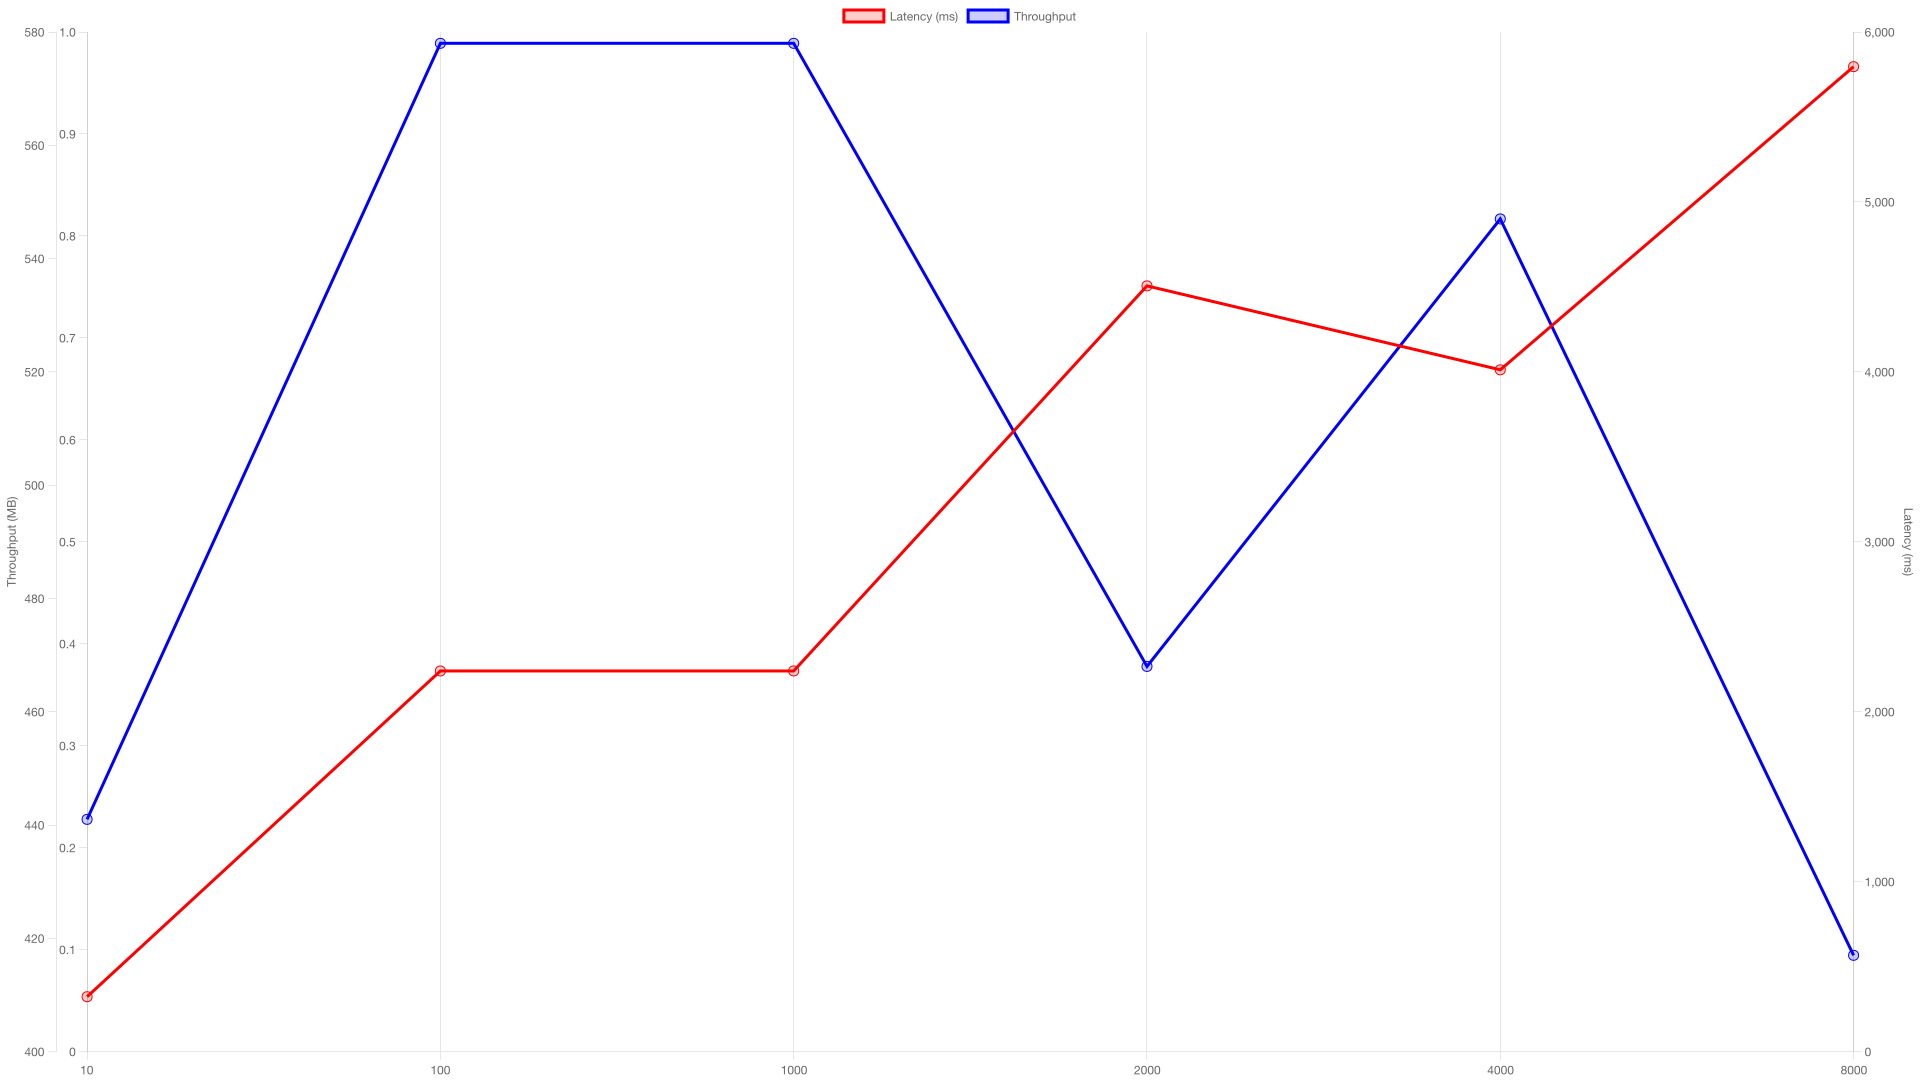
\includegraphics[scale=0.22]{Figure/assignkeycommitment-line-chart.png}
  \caption{AssignKeyCommitment request latency and throughput line chart}
  \label{fig:assignkeycommitment-line-chart}
\end{figure}

The provided dataset comprises performance metrics for various connection types, ranging from ten to eight thousand connections. These metrics are essential for evaluating the system's efficacy and comprehending its behavior under different load conditions. The 2.5th percentile latency ranges from approximately 285 milliseconds to 1162 milliseconds, indicating that only a small percentage of requests experience extremely fast response times. The median latency (50th percentile) ranges between 305 and 2633 milliseconds, representing typical response times for the majority of queries. The 97.5th percentile latency ranges between 478 and 3503 milliseconds, representing the response times for the overwhelming majority of requests. In a similar fashion, the 99th percentile latency ranges from 522 ms to 3567 ms, encompassing response times for an even greater proportion of queries, as well as some outliers. The average latency ranges from 323.71 ms to 2549.27 ms, representing the system's response time as a whole. The range of 52.36 to 552.1 ms for the standard deviation of latency illustrates the variation in response times across queries. The maximal latency ranges between 681 and 5960 milliseconds, representing the longest response time observed throughout the analysis. The 1st and 2.5th percentile values for req/sec are generally low, ranging from 43 to 208, indicating that only a small proportion of requests are processed at the slowest rates. The median req/sec values range from 307 to 434, indicating the rate at which fifty percent of requests were processed. The 97.5th percentile req/sec ranges from 339 to 621, indicating the preponderance of requests' processing speed. The range of 304.7 to 362.8 for the average req/sec indicates the system's ability to handle incoming requests. The range of 39.09 to 153.81 for the standard deviation of req/sec demonstrates the variability of processing rates.\\
\indent The 2.5th percentile throughput values are generally low, ranging from 232 kB to 62.2 kB, indicating that some queries have slower data transmission rates. The median throughput, which corresponds to the 50th percentile, ranges from 263 kilobytes to 62.2 kilobytes, representing the average data transmission rate. The 97.5th percentile throughput ranges between 583 kB and 562 kB, representing the data transfer rate for the plurality of requests. The 99th percentile throughput ranges between 669 kB and 899 kB, representing the data transmission rate for a greater proportion of requests. The range of 441 kB to 525 kB for the average throughput provides an overall measure of data transmission efficacy. The range of 56.6 kB to 223 kB for the standard deviation of throughput illustrates the variability of data transmission rates. In conclusion, this comprehensive data analysis illuminates the performance characteristics of the system across various connection types. By comprehending these metrics, system administrators are able to make informed decisions, optimize performance, and guarantee a seamless and effective user experience. In addition, continuous monitoring of these metrics enables the identification of performance constraints and the planning of future scaling and enhancements to effectively meet user demands.

\subsection{AssignKey}
\begin{table}[H]
  \centering
\begin{tabular}{|l|l|l|l|l|l|l|l|}
\hline
\rowcolor[HTML]{f56b00}
\textbf{Stat} & \textbf{2.5\%} & \textbf{50\%} & \textbf{97.5\%} & \textbf{99\%} & \textbf{Avg} & \textbf{Stdev} & \textbf{Max} \\
\hline
Latency & 447 ms & 465 ms & 2193 ms & 2225 ms & 547.96 ms & 343.23 ms & 2230 ms \\
\hline
\rowcolor[HTML]{f56b00}
\textbf{Stat} & \textbf{1\%} & \textbf{2.5\%} & \textbf{50\%} & \textbf{97.5\%} & \textbf{Avg} & \textbf{Stdev} & \textbf{Min} \\
\hline
Req/Sec & 4 & 4 & 20 & 25 & 17.7 & 6.28 & 4 \\
Bytes/Sec & 3.44 kB & 3.44 kB & 17.2 kB & 21.5 kB & 15.2 kB & 5.4 kB & 3.44 kB \\
\hline
\end{tabular}
 \caption{10 connections performance}
 \label{10-connections-performance}
\end{table}

\begin{table}[H]
  \centering
\begin{tabular}{|l|l|l|l|l|l|l|l|}
\hline
\rowcolor[HTML]{f56b00}
\textbf{Stat} & \textbf{2.5\%} & \textbf{50\%} & \textbf{97.5\%} & \textbf{99\%} & \textbf{Avg} & \textbf{Stdev} & \textbf{Max} \\
\hline
Latency & 453 ms & 500 ms & 784 ms & 834 ms & 539.74 ms & 96.42 ms & 1154 ms \\
\hline
\rowcolor[HTML]{f56b00}
\textbf{Stat} & \textbf{1\%} & \textbf{2.5\%} & \textbf{50\%} & \textbf{97.5\%} & \textbf{Avg} & \textbf{Stdev} & \textbf{Min} \\
\hline
Req/Sec & 96 & 96 & 185 & 219 & 180.8 & 35.31 & 96 \\
Bytes/Sec & 82.6 kB & 82.6 kB & 159 kB & 188 kB & 155 kB & 30.4 kB & 82.6 kB \\
\hline
\end{tabular}
 \caption{100 connections performance}
 \label{100-connections-performance}
\end{table}

\begin{table}[H]
  \centering
  \begin{tabular}{|l|l|l|l|l|l|l|l|}
\hline
\rowcolor[HTML]{f56b00}
\textbf{Stat} & \textbf{2.5\%} & \textbf{50\%} & \textbf{97.5\%} & \textbf{99\%} & \textbf{Avg} & \textbf{Stdev} & \textbf{Max} \\
\hline
Latency & 837 ms & 1561 ms & 6822 ms & 8665 ms & 1842.51 ms & 1257.83 ms & 9971 ms \\
\hline
\rowcolor[HTML]{f56b00}
\textbf{Stat} & \textbf{1\%} & \textbf{2.5\%} & \textbf{50\%} & \textbf{97.5\%} & \textbf{Avg} & \textbf{Stdev} & \textbf{Min} \\
\hline
Req/Sec & 68 & 68 & 277 & 387 & 265.9 & 91.27 & 68 \\
Bytes/Sec & 58.5 kB & 58.5 kB & 238 kB & 333 kB & 229 kB & 78.5 kB & 58.5 kB \\
\hline
\end{tabular}
 \caption{1000 connections performance}
 \label{1000-connections-performance}
\end{table}

\begin{table}[H]
\centering
\begin{tabular}{|l|l|l|l|l|l|l|l|}
\hline
\rowcolor[HTML]{f56b00}
\textbf{Stat} & \textbf{2.5\%} & \textbf{50\%} & \textbf{97.5\%} & \textbf{99\%} & \textbf{Avg} & \textbf{Stdev} & \textbf{Max} \\ \hline
Latency (ms) & 1644 ms & 3205 ms & 8045 ms & 8391 ms & 3589.12 ms & 1408.48 ms & 9823 ms \\ \hline
\rowcolor[HTML]{f56b00}
\textbf{Stat} & \textbf{1\%} & \textbf{2.5\%} & \textbf{50\%} & \textbf{97.5\%} & \textbf{Avg} & \textbf{Stdev} & \textbf{Min} \\ \hline
Req/Sec & 4 & 4 & 360 & 536 & 347.1 & 142.23 & 4 \\ \hline
Bytes/Sec & 3.64 kB & 3.64 kB & 328 kB & 488 kB & 316 kB & 129 kB & 3.64 kB \\ \hline
\end{tabular}
 \caption{2000 connections performance}
 \label{2000-connections-performance}
\end{table}


\begin{table}[H]
\centering
\begin{tabular}{|l|l|l|l|l|l|l|l|}
\hline
\rowcolor[HTML]{f56b00}
\textbf{Stat} & \textbf{2.5\%} & \textbf{50\%} & \textbf{97.5\%} & \textbf{99\%} & \textbf{Avg} & \textbf{Stdev} & \textbf{Max} \\ \hline
Latency (ms) & 2168 ms & 3930 ms & 8805 ms & 9295 ms & 4506.56 ms & 1746.61 ms & 10174 ms \\ \hline
\rowcolor[HTML]{f56b00}
\textbf{Stat} & \textbf{1\%} & \textbf{2.5\%} & \textbf{50\%} & \textbf{97.5\%} & \textbf{Avg} & \textbf{Stdev} & \textbf{Min} \\ \hline
Req/Sec & 0 & 0 & 392 & 628 & 360.8 & 199.87 & 53 \\ \hline
Bytes/Sec & 0 B & 0 B & 357 kB & 572 kB & 328 kB & 182 kB & 48.2 kB \\ \hline
\end{tabular}
 \caption{4000 connections performance}
 \label{4000-connections-performance}
\end{table}

\begin{table}[H]
\centering
\begin{tabular}{|l|l|l|l|l|l|l|l|}
\hline
\rowcolor[HTML]{f56b00}
\textbf{Stat} & \textbf{2.5\%} & \textbf{50\%} & \textbf{97.5\%} & \textbf{99\%} & \textbf{Avg} & \textbf{Stdev} & \textbf{Max} \\ \hline
Latency (ms) & 2652 ms & 5541 ms & 10021 ms & 10150 ms & 5999.93 ms & 2079.53 ms & 10862 ms \\ \hline
\rowcolor[HTML]{f56b00}
\textbf{Stat} & \textbf{1\%} & \textbf{2.5\%} & \textbf{50\%} & \textbf{97.5\%} & \textbf{Avg} & \textbf{Stdev} & \textbf{Min} \\ \hline
Req/Sec & 0 & 0 & 304 & 664 & 297.4 & 198.39 & 4 \\ \hline
Bytes/Sec & 0 B & 0 B & 277 kB & 605 kB & 271 kB & 181 kB & 3.64 kB \\ \hline
\end{tabular}
 \caption{8000 connections performance}
 \label{8000-connections-performance}
\end{table}

\begin{figure}[H]
  \centering
  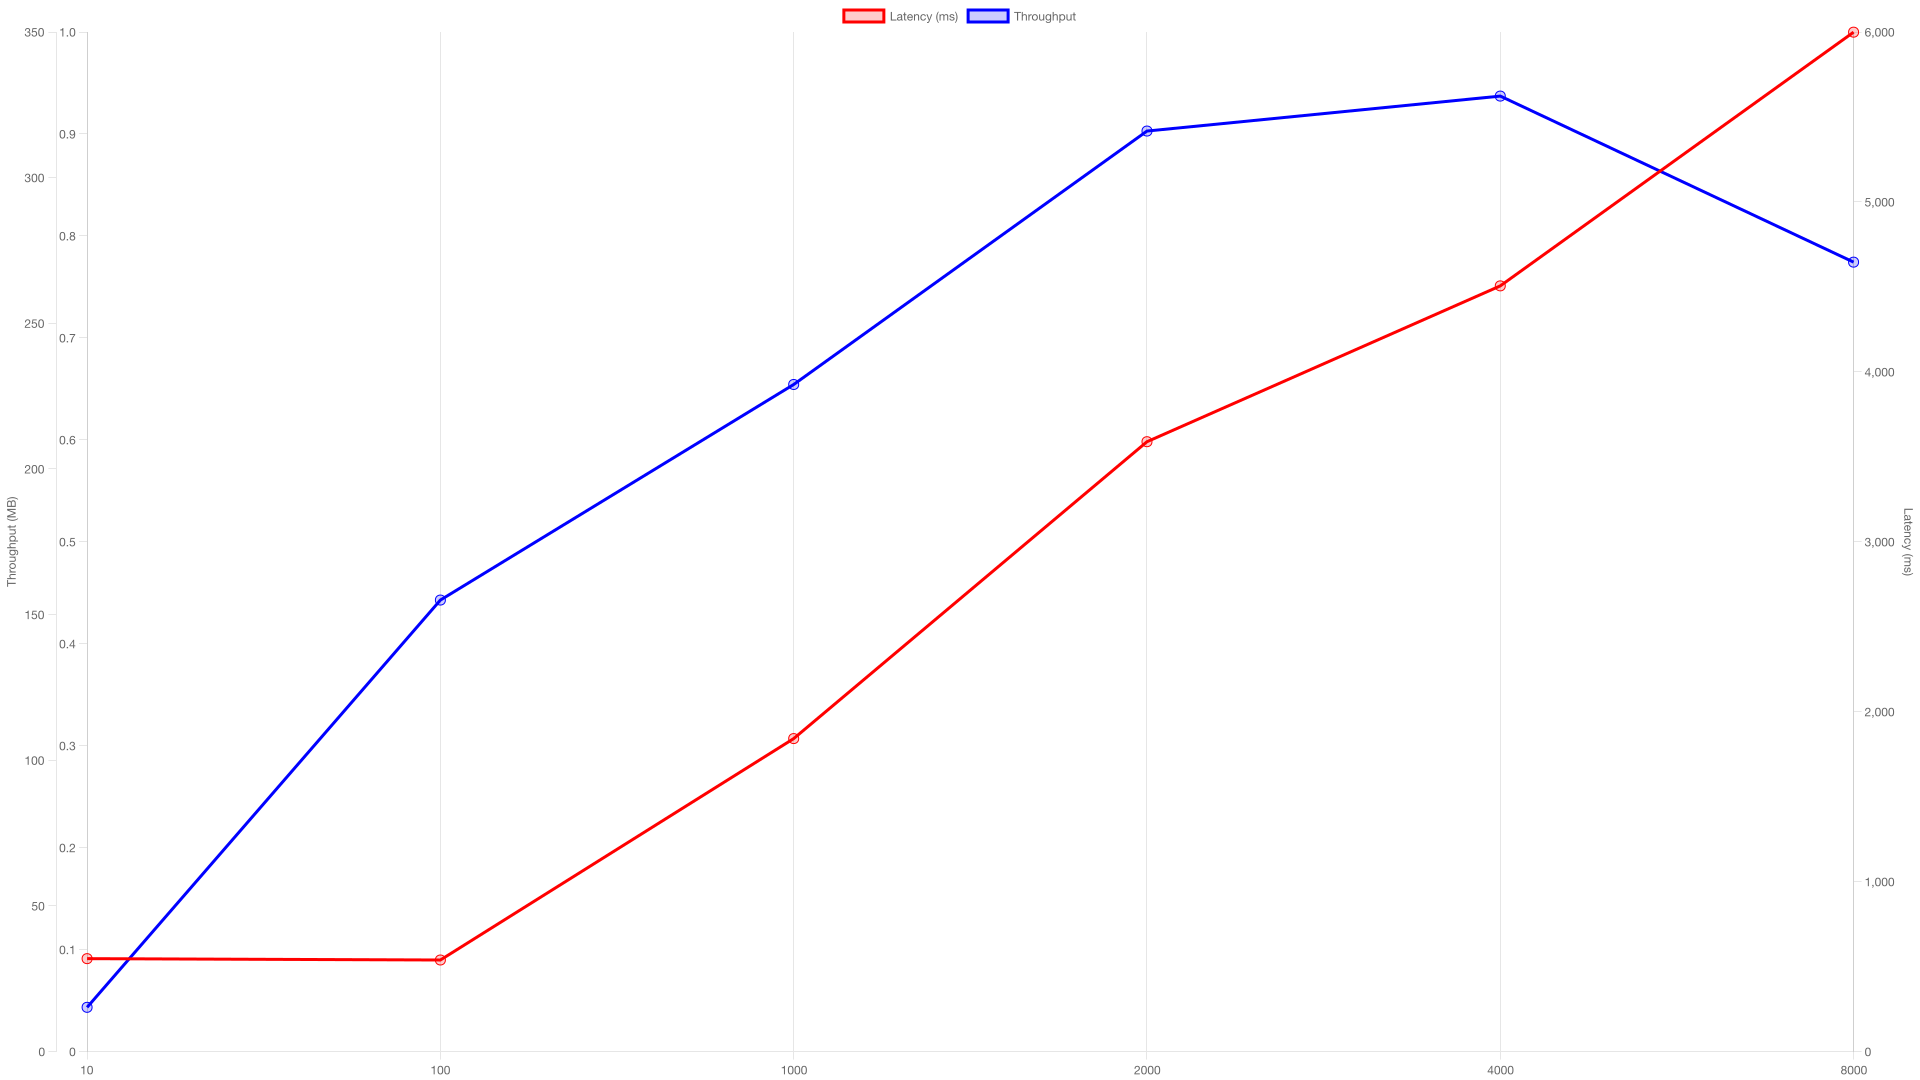
\includegraphics[scale=0.22]{Figure/assignkey-line-chart.png}
  \caption{AssignKey request latency and throughput line chart}
  \label{fig:assignkey-line-chart}
\end{figure}

The median latency for 1000 connections is 1561 milliseconds, whereas the 2.5th percentile latency is approximately 837 milliseconds. The 97.5th and 99th percentile latencies are 6822 ms and 8665 ms, indicating response times for the overwhelming majority of requests. The mean latency is 1842.51 ms and the standard deviation is 1257.83 ms. This instance reveals a maximal latency of 9971 milliseconds.For 2000 connections, the 2.5th percentile latency is approximately 1644 milliseconds, while the 50th percentile latency is approximately 3205 milliseconds. 97.5 percentile and 99 percentile latencies are 8045 and 8391 milliseconds, respectively. Average latency for 2000 connections is 3589.12 ms, with a standard deviation of 1408.48 ms. The longest recorded latency is 9823 milliseconds. The 2.5th percentile latency for 4000 connections is approximately 2168 ms, whereas the 50th percentile latency is approximately 3930 ms. The 97.5th percentile and 99th percentile latencies are 8805 and 9295 milliseconds, respectively. The average latency for 4000 connections is 4506.56 ms, with a standard deviation of 1746.61 ms. 10174 milliseconds is the greatest observed latency in this scenario.\\
\indent The median throughput for 1000 connections is 58.5 kB, with the 2.5th percentile throughput being approximately 58.5 kB. The throughputs for the 97.5th and 99th percentiles are 238 kB and 333 kB, respectively. The average throughput for 1000 connections is 229 kilobytes, with a standard deviation of 78.5 kilobytes. The highest throughput measured is 58.5 kB. For 2000 connections, the 2.5th percentile throughput is approximately 3.64 kilobytes, while the 50th percentile throughput is also 3.64 kilobytes. The throughputs for the 97.5th and 99th percentiles are 328 kB and 488 kB, respectively. The standard deviation for 2000 connections is 129 kB, while the average throughput is 316 kB. 3.64 kB is the maximum throughput observed. The median and 2.5th percentile throughputs for 4000 connections are both 0 bytes, signifying extremely low or no throughput. The throughputs for the 97.5th and 99th percentiles are 357 kB and 572 kB, respectively. The standard deviation of the average throughput for 4000 connections is 182 kB. Maximum throughput measured in this instance is 48.2 kilobytes.\\

\section{Discussion}
Web3Auth is a decentralized oracle network that exhibits similarities with the thesis project. The system also incorporates Shamir's Secret Sharing and DKG (Distributed Key Generation) protocol. Web3Auth provides various key features, as follows:
\begin{itemize}
  \item \textbf{Seamless onboarding}-Web3Auth uses social login to allow users to sign up for dapps with just a few clicks. This makes it easy for users to get started with dapps, and it also helps to improve the user experience.
  \item \textbf{Multi-party computation (MPC)}-Web3Auth uses MPC to provide a secure and private way for users to share their keys. This allows users to collaborate on dapps without having to reveal their private keys. MPC is a cryptographic protocol that allows multiple parties to jointly compute a function without revealing their individual inputs. This makes it a very secure way for users to share their keys, as only the final result of the computation is revealed.

\end{itemize}

\indent Web3Auth has the following disadvantages:
\begin{itemize}
  \item The implementation of nodes for constructing keys of Web3Authen is complex due to the presence of multiple layers within its structure.
  \item The persistence of user data is not guaranteed due to the storage of metadata in a database. If the organization fails to manage this properly, it can result in the loss of information, leading to significant damages.
  \item Web3Auth is not yet widely adopted by dapps, so users may not be able to use their Web3Auth keys on all of the dapps that they want to use. This is because the platform is still relatively new, and it is not yet as widely integrated with dapps as other platforms, such as MetaMask.
  \item To successfully execute projects, various infrastructure components must be operational, with particular emphasis on the node's involvement in registering and creating encryption keys. Scaling out can result in significant infrastructure costs.
\end{itemize}
\indent The system advantages:
\begin{itemize}
  \item By utilizing smart contracts and blockchain technology, user data can be stored and secured in a decentralized manner, guaranteeing its durability and security as long as the blockchain network remains operational.
  \item By transferring the responsibility of constructing encKey and assignKey to the smart contract, the need for implementing intricate nodes to handle consensus between nodes, such as Web3Auth, is eliminated.
  \item The system's complexity decreased, resulting in significant reductions in infrastructure and debugging costs.
\end{itemize}

\end{document}
